\documentclass[11pt, a4paper]{article}
\usepackage{subfiles}

% Algorithms
	%\usepackage{algpseudocode}
	%\usepackage{algorithm}

% Babel
\usepackage[english]{babel}

% Code writing
	%\usepackage[procnames]{listings}

% Font
\usepackage[utf8]{inputenc}
\usepackage[T1]{fontenc}
\usepackage{amssymb,amsmath,amsthm,amsfonts}
\usepackage{eucal}
\usepackage{textcomp}

% Footnote


% Hyperref
\usepackage[hyphens]{url}
\usepackage{cite}
\usepackage{hyperref}
\usepackage{nameref}
\usepackage{url}
% Images
\usepackage[pdftex]{graphicx}
	%\usepackage{subfigure}
\usepackage{subfig}
\usepackage{eso-pic}
\usepackage{caption}
\usepackage{wrapfig}
\usepackage{float}

% List
\usepackage{enumerate}

% SI units
\usepackage{siunitx}

% Standalone
\usepackage[subpreambles=true]{standalone}
\usepackage{import}

% Tables
\usepackage{tabularx}
\usepackage{booktabs}
\usepackage{multirow}

% TiKz and graphs
\usepackage{pgf,tikz,pgfplots}
% \usepackage{gnuplottex}
\usepackage{bm}
\usepackage{relsize}
%\usepackage[compat=1.1.0]{tikz-feynman}
\usepackage{circuitikz}

% Typeset
%\usepackage[top=2cm,bottom=2cm,left=2cm,right=2cm]{geometry}
\usepackage[top=2cm,bottom=2cm,left=2cm,right=2cm]{geometry}
\usepackage{fancyhdr}
\usepackage{indentfirst}
\usepackage{titlesec}
\usepackage{setspace}
\usepackage{xspace}
% \usepackage{parskip}  % Elimina il separatore a inizio paragrafo
\usepackage{afterpage}
\usepackage{comment}

%Python
\usepackage{xcolor}
\usepackage{listings}
\usepackage{framed}

%Per scrivere matrice identità
\usepackage{bbold}
%Per semplificazione formule
\usepackage{cancel}

%Evidenziare formule
\usepackage{empheq}
	%oppure
	%\usepackage{xcolor}
\usepackage{soul}

%Evidenziare testo con mdframed
\usepackage{mdframed}

%Note a margine
\usepackage{marginnote}

%Display data
\usepackage{datetime}

%Physics
\usepackage{physics}

%Geometry
%\newgeometry{inner=20mm,
%            outer=49mm,% = marginparsep + marginparwidth
%                       %   + 5mm (between marginpar and page border)
%            top=20mm,
%            bottom=25mm,
%            marginparsep=6mm,
%            marginparwidth=30mm}
%\makeatletter
%\renewcommand{\@marginparreset}{%
%  \reset@font\small
%  \raggedright
%  \slshape
%  \@setminipage
%}
%\makeatother

%Atom Latex
%\pgfplotsset{compat=1.15}

%%
\captionsetup[table]{font=small,labelfont={bf},skip=10pt}
\captionsetup[figure]{font=small,labelfont={bf},skip=10pt}

%intestazione pagina
%\pagestyle{fancy}
%\fancyhf{}
%\fancyhead[RE]{\ifnum\value{chapter}>0\nouppercase{\leftmark}\fi}
%\fancyhead[LE]{\small\textbf{\thepage}}
%\fancyhead[LO]{\nouppercase{\rightmark}}
%\fancyhead[RO]{\small\textbf{\thepage}}

%link ipertestuale per indice
\hypersetup{
	colorlinks=false,
	linkcolor=black,
	filecolor=blue,
	citecolor = blue,
	urlcolor=blue,
	}

%%%%%indent%%%
\setlength{\parindent}{15pt}
\setlength{\parskip}{0pt}


%boh
%\renewcommand{\chaptermark}[1]{%
% \markboth{\MakeUppercase{%
% \chaptername}\ \thechapter.%
% \ #1}{}}


 %Python in latex
 \definecolor{codegreen}{rgb}{0,0.6,0}
\definecolor{codegray}{rgb}{0.5,0.5,0.5}
\definecolor{codepurple}{rgb}{0.58,0,0.82}
\definecolor{backcolour}{rgb}{0.95,0.95,0.92}
\definecolor{commentcolour}{rgb}{0.43,0.63,0.65}

\definecolor{shadecolor}{rgb}{0.93, 0.93, 0.93}
\definecolor{darkgreen}{rgb}{0.0, 0.5, 0.0}
\definecolor{darkred}{rgb}{0.8, 0.0, 0.0}
\definecolor{violet}{rgb}{0.55, 0.0, 0.55}

\lstdefinestyle{mystyle}{ %Stile python code
    backgroundcolor=\color{shadecolor},
    commentstyle=\color{commentcolour},
    keywordstyle=\color{darkgreen},
    numberstyle=\tiny\color{codegray},
    stringstyle=\color{darkred},
    basicstyle=\ttfamily\footnotesize,
    breakatwhitespace=false,
    breaklines=true,
    captionpos=b,
    keepspaces=true,
    numbers=left,
    numbersep=5pt,
    showspaces=false,
    showstringspaces=false,
    showtabs=false,
    tabsize=2
}

\lstset{style=mystyle}

%VHDL in latex
\usepackage{beramono}
\lstdefinelanguage{VHDL}{
   morekeywords={
     library,use,all,entity,is,port,in,out,end,architecture,of,
     begin,and
   },
   morecomment=[l]--
}
\colorlet{keyword}{blue!100!black!80}
\colorlet{comment}{green!90!black!90}
\lstdefinestyle{vhdl}{
   language     = VHDL,
   basicstyle   = \ttfamily\footnotesize,
   keywordstyle = \color{keyword}\bfseries,
   commentstyle = \color{comment}
}


% Derivatives
\renewcommand{\d}[0]{\mathrm{d}}
\newcommand{\dev}[2]{\displaystyle \frac{\d #1}{\d #2}}
\newcommand{\pdev}[2]{\displaystyle \frac{\partial #1}{\partial #2}}
\newcommand{\ndev}[3]{\displaystyle \frac{\d^{#3} #1}{\d #2^{#3} } }
\newcommand{\npdev}[3]{\displaystyle \frac{\partial^{#3} #1}{\partial #2^{#3} } }


%% Norms
\newcommand{\absvec}[1]{| \vec{#1} |}
\newcommand{\normvec}[1]{|\!| \vec{#1} |\!|}

\newcommand{\vmed}[1]{\left \langle #1 \right \rangle}
\newcommand{\vmedvec}[1]{\langle #1 \rangle}
\newcommand{\R}[0]{\mathbb{R}}
\renewcommand{\H}[0]{\operatorname{H}}

%Evidenziare formule
\newcommand{\mathcolorbox}[2]{\colorbox{#1}{$\displaystyle #2$}}
\newcommand{\hlfancy}[2]{\sethlcolor{#1}\hl{#2}}

%Theorem
\newtheorem{theorem}{Theorem}[section]
\newtheorem{corollary}{Corollary}[theorem]
\newtheorem{lemma}[theorem]{Lemma}
\newtheorem{proposition}[theorem]{Proposition}

\theoremstyle{definition}
\newtheorem{definition}{Definition}%[section]


%%%%%%%%%%%%%%%%%%%%Exercise and example%%%%%%%%%%%%%%%%%
\usepackage[many,most,theorems]{tcolorbox}


\newtcbtheorem{exercise}{Exercise}{ % frame stuff
    boxrule = 1pt,
    breakable,
    enhanced,
    frame empty,
    interior style= {blue!6},
    %interior empty,
    colframe=black,
    borderline ={1pt}{0pt}{black},
    left=0.2cm,
    % title stuff
    attach boxed title to top left={yshift=-2mm,xshift=0mm},
    coltitle=black,
    fonttitle=\bfseries,
    colbacktitle=white,
    boxed title style={boxrule=1pt,sharp corners}}{exercise} 

\newtcbtheorem{example}{Example}{ % frame stuff
    boxrule = 1pt,
    enhanced,
    frame empty,
    interior style= {green!6},%{left color=yellow!70,right color=green!70},
    %interior empty,
    colframe=black,
    borderline ={1pt}{0pt}{black},
    breakable,
    left=0.2cm,
    % title stuff
    attach boxed title to top left={yshift=-2mm,xshift=0mm},
    coltitle=black,
    fonttitle=\bfseries,
    colbacktitle=white,
    boxed title style={boxrule=1pt,sharp corners}}{example}
  
%\newtheorem{exercise}{Exercise}
%\newtheorem{example}{Example}

%%%%%%%%%%%%%%%%%%%%%%%%%%%%%%%%%%%

\theoremstyle{remark}
\newtheorem*{remark}{Remark}
\newtheorem{observation}{Observation}
%Evidenziare testo
\newtheorem*{solution}{Solution}

\newcommand\mybox[1]{%
  \fbox{\begin{minipage}{0.9\textwidth}#1\end{minipage}}}

  %Spiegazioni/verifiche
\newenvironment{greenbox}{\begin{mdframed}[hidealllines=true,backgroundcolor=green!20,innerleftmargin=3pt,innerrightmargin=3pt,innertopmargin=3pt,innerbottommargin=3pt]}{\end{mdframed}}

\newenvironment{bluebox}{\begin{mdframed}[hidealllines=true,backgroundcolor=blue!10,innerleftmargin=3pt,innerrightmargin=3pt,innertopmargin=3pt,innerbottommargin=3pt]}{\end{mdframed}}

\newenvironment{yellowbox}{\begin{mdframed}[hidealllines=true,backgroundcolor=yellow!20,innerleftmargin=3pt,innerrightmargin=3pt,innertopmargin=3pt,innerbottommargin=3pt]}{\end{mdframed}}

\newenvironment{redbox}{\begin{mdframed}[hidealllines=true,backgroundcolor=red!20,innerleftmargin=3pt,innerrightmargin=3pt,innertopmargin=3pt,innerbottommargin=3pt]}{\end{mdframed}}

\newenvironment{orangebox}{\begin{mdframed}[hidealllines=true,backgroundcolor=orange!20,innerleftmargin=3pt,innerrightmargin=3pt,innertopmargin=3pt,innerbottommargin=3pt]}{\end{mdframed}}

%emph equation
\newcommand*\myyellowbox[1]{%
  \colorbox{yellow!40}{\hspace{1em}#1\hspace{1em}}}

\newcommand*\mygreenbox[1]{%
  \colorbox{green!20}{\hspace{1em}#1\hspace{1em}}}
  
  
  
  
  


\begin{document}

\author{Rocco Ardino\\1231629  \and Alessandro Lambertini\\ 1242885 \and Alice Pagano \\1236916 \and Michele Puppin \\ 1227474}
\title{\textbf{Management and Analysis of Physics Dataset (mod. A): \\ FIR filter co-processor in FPGA with IPbus protocol}}
\maketitle

\section{Aim}
In this project we implement a FIR filter co-processor in FPGA, along with input/output data storage and transfer protocols. In particular, we use the IPbus protocol for communication with the FPGA board and a DPRAM component as memory source. We test the hardware implementation of the filter on several input waveforms and we compare the results with the ones obtained through a Python simulation.





\section{Implementation}
We send data to be filtered from the PC to the FPGA, connected with an Ethernet cable, through the IPbus protocol. Then, data are stored in FPGA memory registers and we use DPRAM to read data from memory. We apply the FIR filter and we store back filtered data using again DPRAM. A cartoon of the entire process is schematized in Fig.\ref{fig:first_diagram}. Eventually, we make use of a Python script in order to interface with the FPGA via IPbus.

\vspace{1cm}
\begin{figure}[h!]
    \centering
    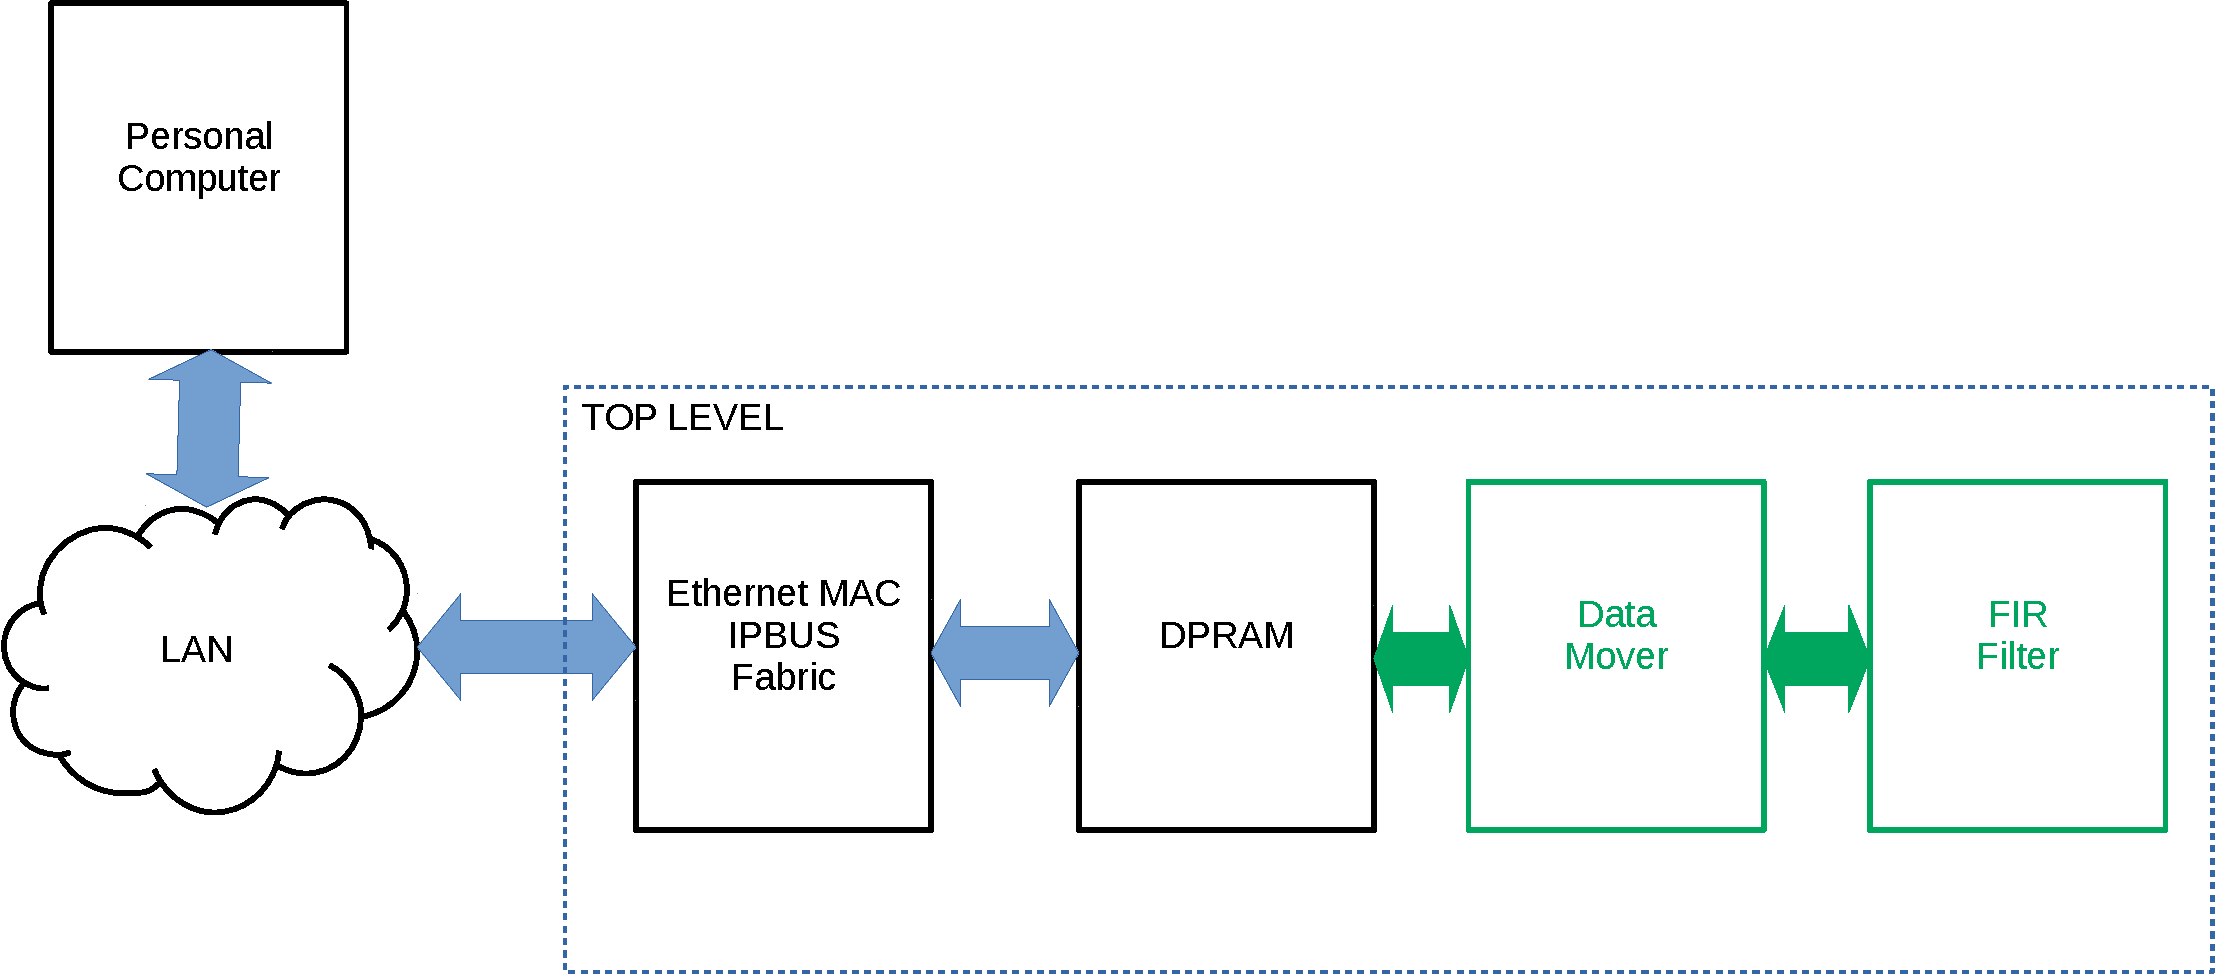
\includegraphics[width=0.8\textwidth]{../images/implementation/diagram.pdf}
    \caption{\label{fig:first_diagram} Diagram of implemented FIR filter co-processor in FPGA with IPbus protocol.}
\end{figure}
\vspace{1cm}

Now, we describe in details the structure of the main components and the finite state machine we implement to interface the DPRAM with the FIR filter.

\subsection{DPRAM}
By definition, a DPRAM is a type of random-access memory that allows multiple reads or writes to occur at the same time. Its VHDL IPbus based implementation is showed in Listing \ref{lst:ipbus_dpram} and the main ports are explained below:
\begin{itemize}
    \item {\footnotesize\texttt{we}}: write/read flag. If set to `0', the DPRAM is in read mode; otherwise it is in write mode.
    \item {\footnotesize\texttt{d}}: data to be written to a specified address of the DPRAM.
    \item {\footnotesize\texttt{q}}: data to be read from a specified address of the DPRAM.
    \item {\footnotesize\texttt{addr}}: address of the DPRAM in which read/write operations are executed.
\end{itemize}

\begin{lstlisting}[style=vhdl,label={lst:ipbus_dpram},caption={{\footnotesize\texttt{ipbus\_dpram}} entity.}]
entity ipbus_dpram is
	generic( ADDR_WIDTH: natural );
	port(
		clk     : in  std_logic;
		rst     : in  std_logic;
		ipb_in  : in  ipb_wbus;
		ipb_out : out ipb_rbus;
		rclk    : in  std_logic;
		we      : in  std_logic := '0';
		d       : in  std_logic_vector(31 downto 0) := (others => '0');
		q       : out std_logic_vector(31 downto 0);
		addr    : in  std_logic_vector(ADDR_WIDTH - 1 downto 0) );
end ipbus_dpram;
\end{lstlisting}

In particular, the ``reading from'' and ``writing to'' process is displayed in Listing \ref{lst:dpram_process}. At every cycle of the DPRAM clock signal {\footnotesize\texttt{rclk}}, we access to the specified address of the DPRAM by index. Then, if {\footnotesize\texttt{we}} is `0', we read from it, otherwise we write to it.

\begin{lstlisting}[style=vhdl,label={lst:dpram_process},caption={Read from/Write to DPRAM process.}]
rsel <= to_integer(unsigned(addr));

process(rclk)
begin
	if rising_edge(rclk) then
		q <= ram(rsel); 
		if we = '1' then
			ram(rsel) := d;
		end if;
	end if;
end process;
\end{lstlisting}

\noindent
In our {\footnotesize\texttt{top\_level}} entity we instantiate the IPbus based DPRAM as represented in Listing \ref{lst:ipbus_dpram_instantiation}. 

\begin{lstlisting}[style=vhdl,label={lst:ipbus_dpram_instantiation},caption={{\footnotesize\texttt{ipbus\_dpram}} instantiation in the {\footnotesize\texttt{top\_level}}.}]
-- Flash registers
dpram : ipbus_dpram
	generic map(ADDR_WIDTH => ADDR_WIDTH)
	port map(
		clk     => ipb_clk,
		rst     => rst_ipb,
		ipb_in  => ipbw(0),
		ipb_out => ipbr(0),
		rclk    => ipb_clk,
		we      => we_s,
		d       => data_out,	--data to write
		q       => data_in,		--data to read
		addr    => addr_s);
\end{lstlisting}



\subsection{FIR Filter}
We implement a finite impulse response (FIR) filter, which is a filter whose impulse response is of finite duration.
%%%
Firstly, we provide a brief mathematical introduction. Given a sequence $\{x_i\}_{i=1,\dots,N}$ of $N$ input data samples, the output sequence of the filter is obtained by applying the following operation:
\begin{equation}
    \begin{aligned}
        y[n] &=b_{0} x[n]+b_{1} x[n-1]+\cdots+b_{k-1} x[n-k+1] \\
        &=\sum_{i=0}^{k-1} b_{i} \cdot x[n-i]
    \end{aligned}
    \label{eq:FIR}
\end{equation}
which is a convolution operation, or more simply, a weighted moving average. The $b_i$ in Eq. \ref{eq:FIR} are the coefficients that characterize the filter and its order. So, a $k$-th order filter is a filter that works with $k$ coefficients.

%More specifically, the impulse response of f a \(N\)-th order discrete-time FIR filter lasts exactly \(N+1\) samples. Concerning the order of the filter itself, it is defined by the nu

%For a causal discrete-time FIR filter of order $N$, each value of the output sequence is a weighted sum of the most recent input values:
%\begin{equation}
%    \begin{aligned}
%        y[n] &=b_{0} x[n]+b_{1} x[n-1]+\cdots+b_{N} x[n-N] \\
%        &=\sum_{i=0}^{N} b_{i} \cdot x[n-i]
%    \end{aligned}
%\end{equation}
%where the $b_i$ are the coefficients of the filter itself.

%For our aims
In our work, we consider a 5-th order FIR filter. The values of the coefficients are computed through the library \textit{signal} of the Python module \textit{scipy}, by setting a cutoff frequency of $0.1$. The frequency analysis for this filter setup is showed in Figure \ref{fig:FIR_freq_analysis}.

\begin{figure}[!h]
    \centering
    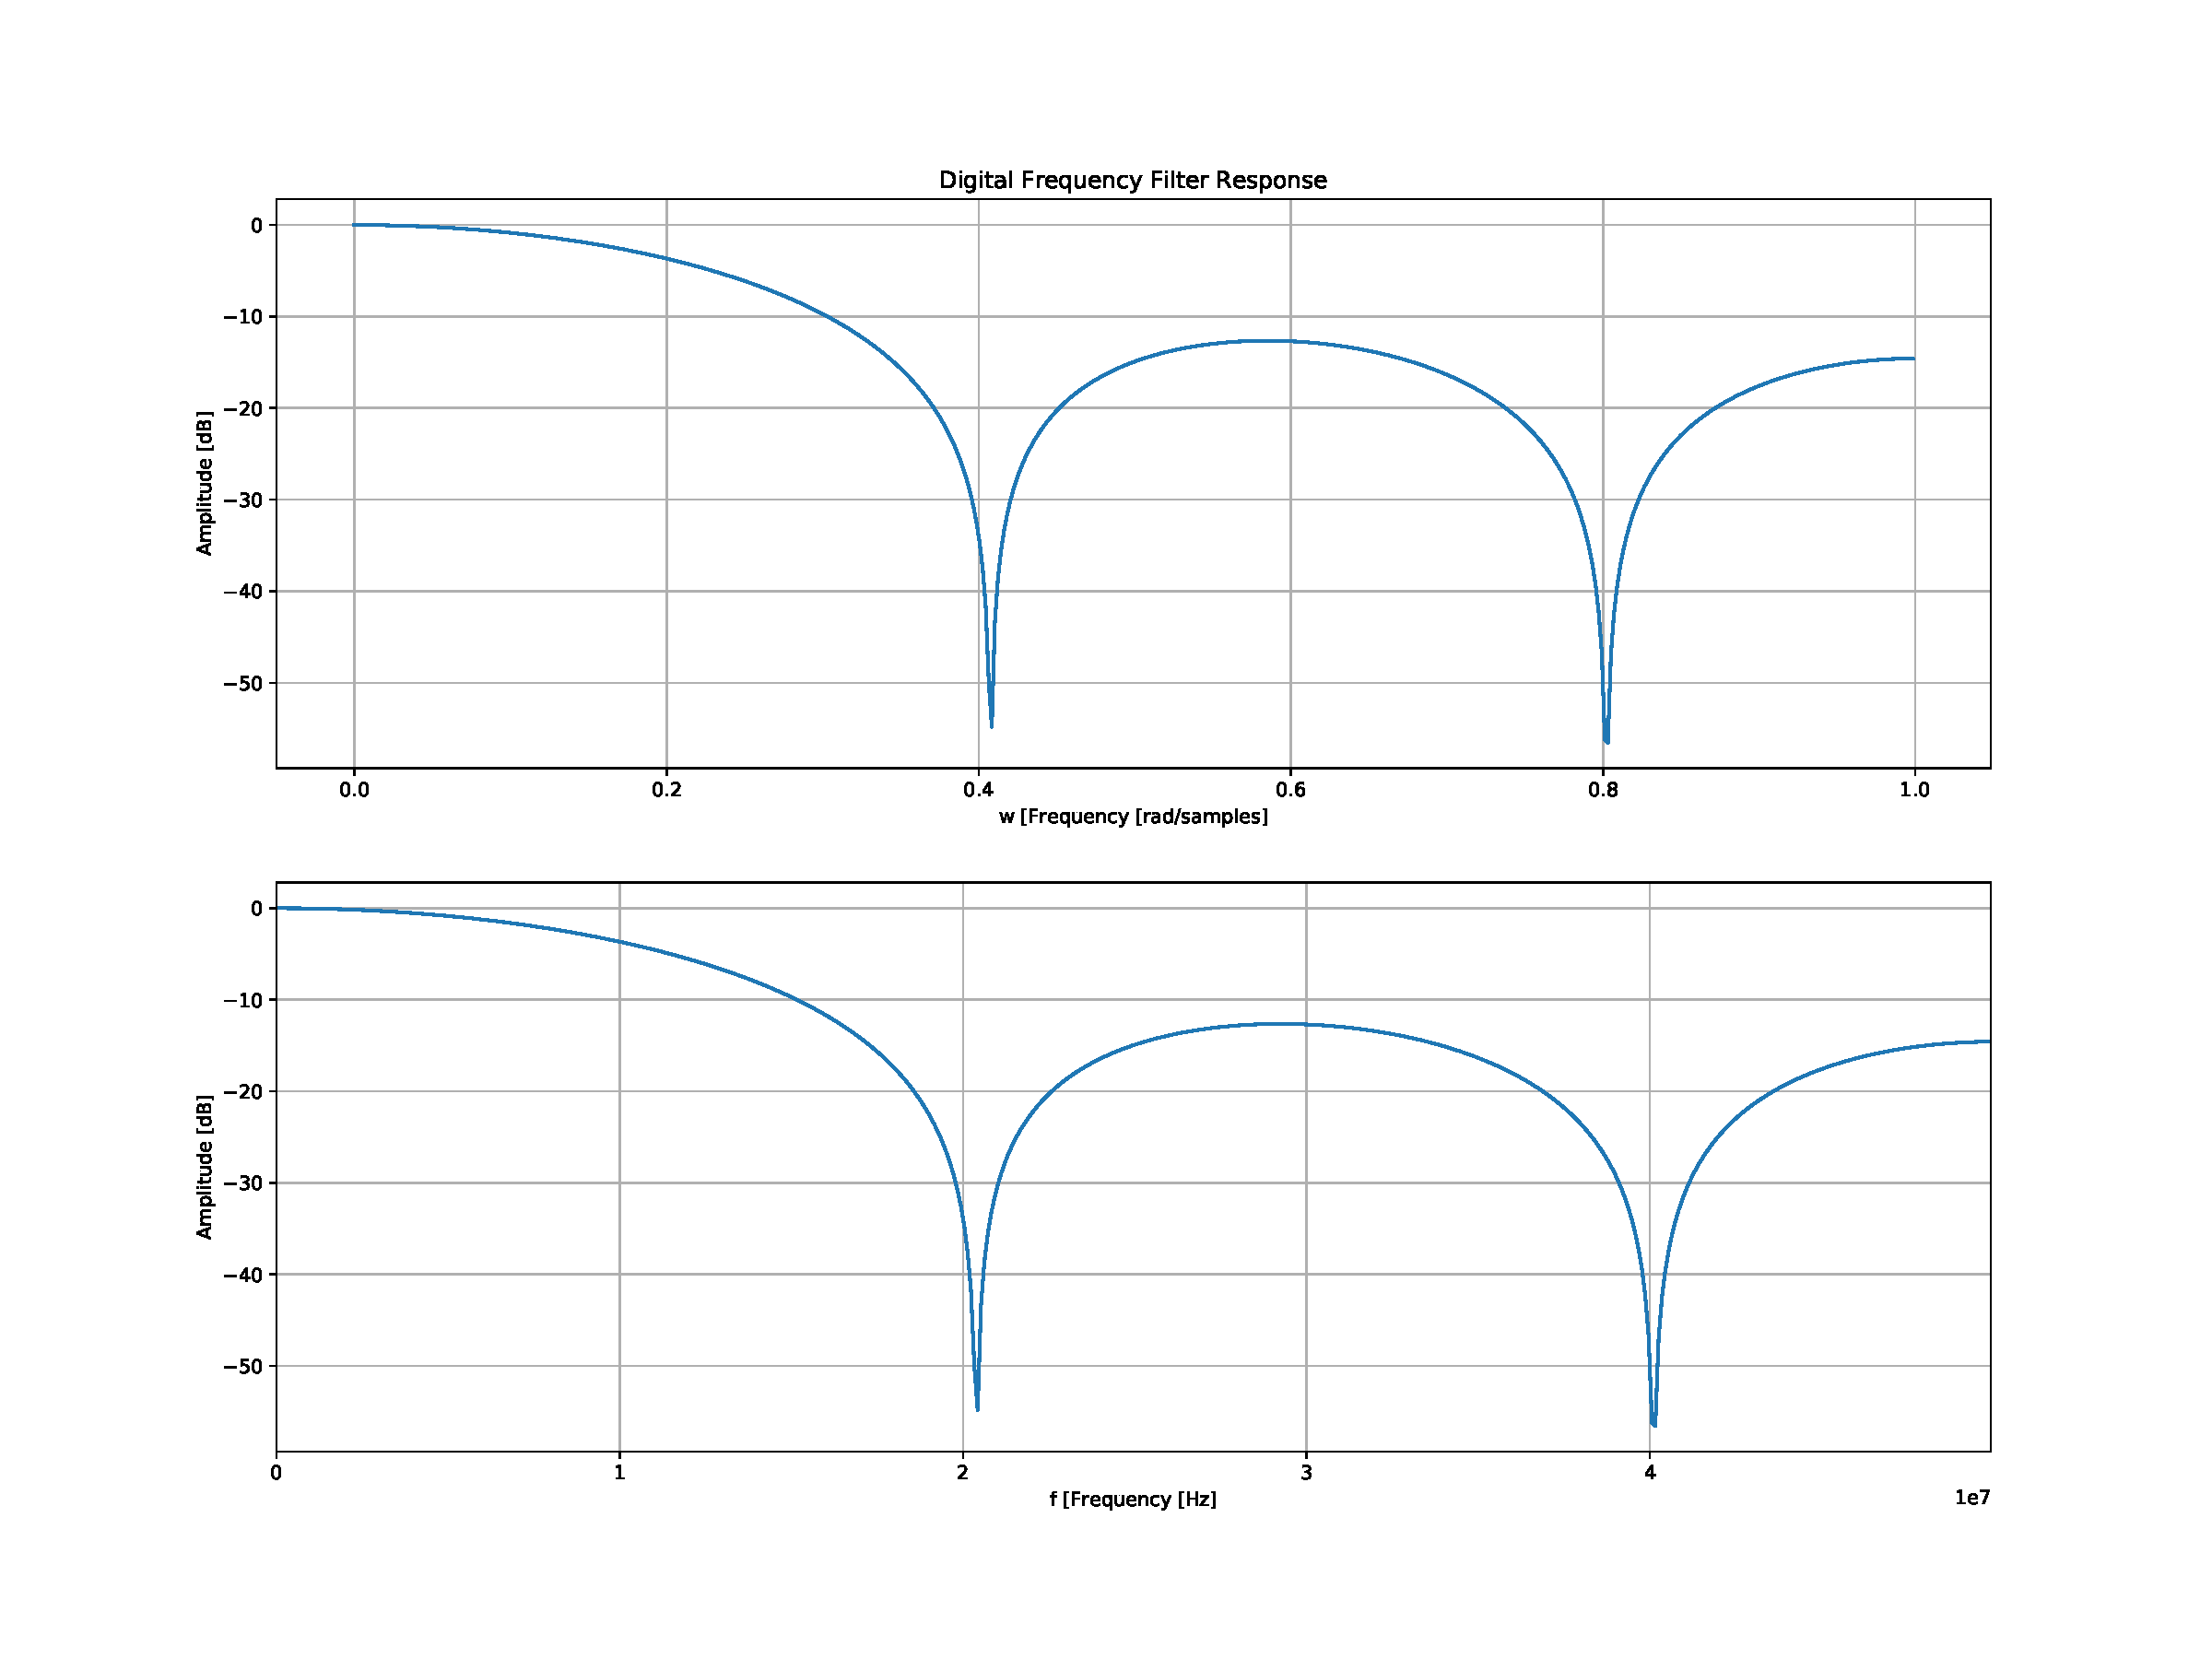
\includegraphics[width=1.0\textwidth]{../images/implementation/FIR_filter_freq_analysis.pdf}
    \caption{Frequency analysis of the FIR filter with the given configuration.}
    \label{fig:FIR_freq_analysis}
\end{figure}

The values of the coefficients are:
\begin{align*}
    b_0 &= 0.1933  \\
    b_1 &= 0.2033  \\
    b_2 &= 0.2066  \\
    b_3 &= 0.2033  \\
    b_4 &= 0.1933
\end{align*}
Since every operation on the FPGA is done with integer arithmetics, it is fundamental to overcome the limit of the finite precision of those coefficients. An idea is to multipilicate them by a large number such $10^3$ and then truncate the floating part. Hence, the values of the coefficients in the VHDL code are set to:
\begin{align*}
    b_0 &= \mathrm{193}_{\text{dec}}  \qquad \Longrightarrow \qquad \mathrm{000000C1}_{\text{hex}}   \\
    b_1 &= \mathrm{203}_{\text{dec}}  \qquad \Longrightarrow \qquad \mathrm{000000CB}_{\text{hex}}   \\
    b_2 &= \mathrm{206}_{\text{dec}}  \qquad \Longrightarrow \qquad \mathrm{000000CE}_{\text{hex}}   \\
    b_3 &= \mathrm{203}_{\text{dec}}  \qquad \Longrightarrow \qquad \mathrm{000000CB}_{\text{hex}}   \\
    b_4 &= \mathrm{193}_{\text{dec}}  \qquad \Longrightarrow \qquad \mathrm{000000C1}_{\text{hex}}
\end{align*}














\subsection{Finite State Machine}
In order to interface the FIR filter with the DPRAM, we implement a finite state machine able to perform read, filter and write operations. In particular, we define the entity {\footnotesize\texttt{fir\_filter}} in Listing \ref{lst:fir_filter} and the main ports are explained below:
\begin{itemize}
    \item {\footnotesize\texttt{i\_coeff\_*}}: coefficients of the FIR filter.
    \item {\footnotesize\texttt{we\_out}}: write/read flag. If set to `0', the state machine enables data read operation; otherwise it enables data write operations.
    \item {\footnotesize\texttt{x\_in}}: input data in \(32\)-bit format.
    \item {\footnotesize\texttt{y\_out}}: output data in \(32\)-bit format.
    \item {\footnotesize\texttt{address}}: address where input and output data are read or written.
\end{itemize}

\begin{lstlisting}[style=vhdl,label={lst:fir_filter},caption={{\footnotesize\texttt{fir\_filter}} entity.}]
entity fir_filter is
	port (
		clk       : in  std_logic;
		rst       : in  std_logic;
		i_coeff_0 : in  std_logic_vector(31 downto 0);
		i_coeff_1 : in  std_logic_vector(31 downto 0);
		i_coeff_2 : in  std_logic_vector(31 downto 0);
		i_coeff_3 : in  std_logic_vector(31 downto 0);
		i_coeff_4 : in  std_logic_vector(31 downto 0);
		x_in      : in  std_logic_vector(31 downto 0);
		y_out     : out std_logic_vector(31 downto 0);
		we_out    : out std_logic; -- write enable for the dpram
		address   : out std_logic_vector(9 downto 0) );
end fir_filter;
\end{lstlisting}

In the {\footnotesize\texttt{top\_level}} entity we instantiate the component {\footnotesize\texttt{fir\_filter}} as in Listing \ref{lst:fir_filter_instantiation}. In particular, the ports {\footnotesize\texttt{x\_in}}, {\footnotesize\texttt{y\_out}}, {\footnotesize\texttt{we\_out}} and {\footnotesize\texttt{address}} are mapped to the same signals to which {\footnotesize\texttt{q}}, {\footnotesize\texttt{p}}, {\footnotesize\texttt{we\_s}} and {\footnotesize\texttt{addr\_s}} are respectively mapped. Note that clock and reset ({\footnotesize\texttt{clk}} and {\footnotesize\texttt{rst}}) are mapped to the ones of IPbus. 

\begin{lstlisting}[style=vhdl,label={lst:fir_filter_instantiation},caption={{\footnotesize\texttt{fir\_filter}} instantiation in the {\footnotesize\texttt{top\_level}}.}]
fir: fir_filter
	port map (
		clk       => ipb_clk,
		rst       => rst_ipb,
		i_coeff_0 => i_coeff_0,
		i_coeff_1 => i_coeff_1,
		i_coeff_2 => i_coeff_2,
		i_coeff_3 => i_coeff_3,
		i_coeff_4 => i_coeff_4,
		x_in      => data_in,
		y_out     => data_out,
		we_out    => we_s, -- write enable for the dpram
		address   => addr_s );
\end{lstlisting}

In the entity {\footnotesize\texttt{fir\_filter}} we build a process {\footnotesize\texttt{fsm\_fir}} in which the finite state machine is implemented.
We perform read and write operations so that we read from the first half of the memory and we write in the second half, until the memory is full and the process starts again overwriting data. In particular, we define a signal {\footnotesize\texttt{state\_fsm}} which can be one of the following three possible states: {\footnotesize\texttt{s\_idle}},  {\footnotesize\texttt{s\_read}} and {\footnotesize\texttt{s\_write}}. Moreover, we define an integer signal {\footnotesize\texttt{samples}} which is used as a counter of read/write operations.

Initially, the state is set to {\footnotesize\texttt{s\_idle}}  where  {\footnotesize\texttt{we\_out}} and {\footnotesize\texttt{samples}} are set to '0'.
Then, at each rising edge of the clock, the machine switches its state from {\footnotesize\texttt{s\_read}} to {\footnotesize\texttt{s\_write}} or vice versa. 

In case {\footnotesize\texttt{s\_read}} is selected, as showed in Listing \ref{lst:s_read}, read flag is enabled. The integer signal {\footnotesize\texttt{samples}} is converted to the reading address in order to read from the first half of the memory. The data at that address is then read. Eventually, the state is switched to {\footnotesize\texttt{s\_write}}.

\begin{lstlisting}[style=vhdl,label={lst:s_read},caption={Read state of the finite state machine.}]
when s_read =>
    we_out    <= '0';
    address   <= std_logic_vector(to_unsigned(samples, address'length));
    x         <= std_logic_vector(signed(x_in));
    state_fsm <= s_write;
\end{lstlisting}

In case {\footnotesize\texttt{s\_write}} is selected, as shown in Listing \ref{lst:s_write}, write flag is enabled. The writing address is obtained by taking the binary value of the signal {\footnotesize\texttt{samples}} incremented by half of the length of the memory. The data previously read is now filtered and sent to the output variable. Then, the signal {\footnotesize\texttt{samples}} is incremented by one unit. When {\footnotesize\texttt{samples}} reaches \(512\) (i.e. half of the memory length), we reset the counter in order to start the process all over again. 

\begin{lstlisting}[style=vhdl,label={lst:s_write},caption={Write state of the finite state machine.}]
when s_write =>
	we_out <= '1';
	address   <= std_logic_vector(to_unsigned(samples+512, address'length));
	p_data    <= signed(x) & p_data(0 to p_data'length-2);
	y_out     <= std_logic_vector(resize(
                                    p_data(0)*signed(i_coeff_0) +
                                    p_data(1)*signed(i_coeff_1) +
                                    p_data(2)*signed(i_coeff_2) +
                                    p_data(3)*signed(i_coeff_3) +
                                    p_data(4)*signed(i_coeff_4), 32) );
	samples   <= samples + 1;
	if samples = 512 then
		p_data    <= (others => (others => '0'));
		samples   <= 0;
		we_out    <= '0';
		state_fsm <= s_idle;
	else
		state_fsm <= s_read;
	end if;
\end{lstlisting}

%Moreover, as far as it concerns the filter implementation, we have to take into account that the FIR filter has as many transient states as the number of taps. In fact, since the filter needs the four previous data, we need to set up a data pipe to store them. 

Lastly, a consideration must be done on the intrinsic transient states of the filter. Indeed, since the filter needs the four previous data to produce an output value, we need to set up a data pipe to store them at every cycle of the finite state machine. This is done by exploiting the VHDL operator ``{\footnotesize\texttt{\&}}'', which concatenates the new input data to be processed with the first four data of the data pipe. However, this procedure is not well defined for the first four input data in the memory since the data pipe is not completely filled when they are processed. Therefore, the filter will behave as expected after four samples are processed.

Every procedure described before is summarized in the schematics in Figure \ref{fig:wavedrom}.
\clearpage
\begin{figure}[h!]
    \centering
    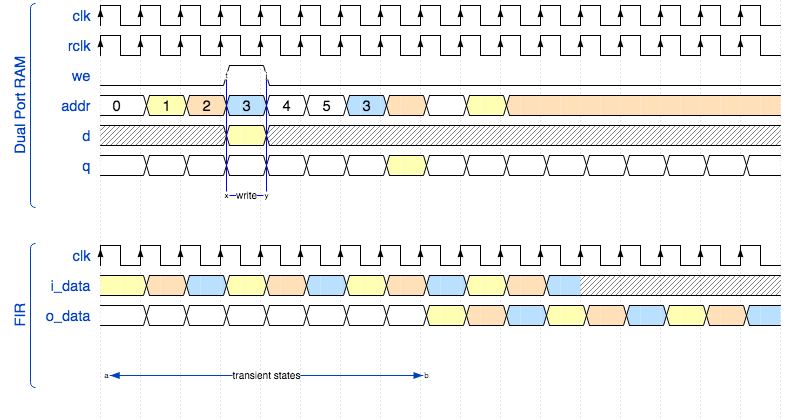
\includegraphics[width=1.0\textwidth]{../images/implementation/wavedrom.png}
    \caption{Summary of the working principles of the whole implemented system.}
    \label{fig:wavedrom}
\end{figure}





\section{Behavioral validation}
First of all, we generate the bitstream and program the device. Then, the Arty7 board is connected to a PC through an Ethernet cable and the IP address is configured. In order to upload data and download filtered data respectively to and from the board, we use the Python API uHAL. 

We send in input several waveforms to test the FIR filter. Moreover, we compare the results using a Python script which uses the same type of filter with the same parameters. 

\subsection{Sine wave input}
The first waveform under study is a sine wave with the following parameters:
\begin{itemize}
    \item amplitude: $A = 1024$;
    \item period: $T = 500 \ \si{samples}$.
\end{itemize}
The results for this waveform are showed in Figure \ref{fig:sine_wave}. As we can see from the plot, the filter behaves as expected, except for the samples corresponding to the initial transient states.
\begin{figure}[h!]
    \centering
    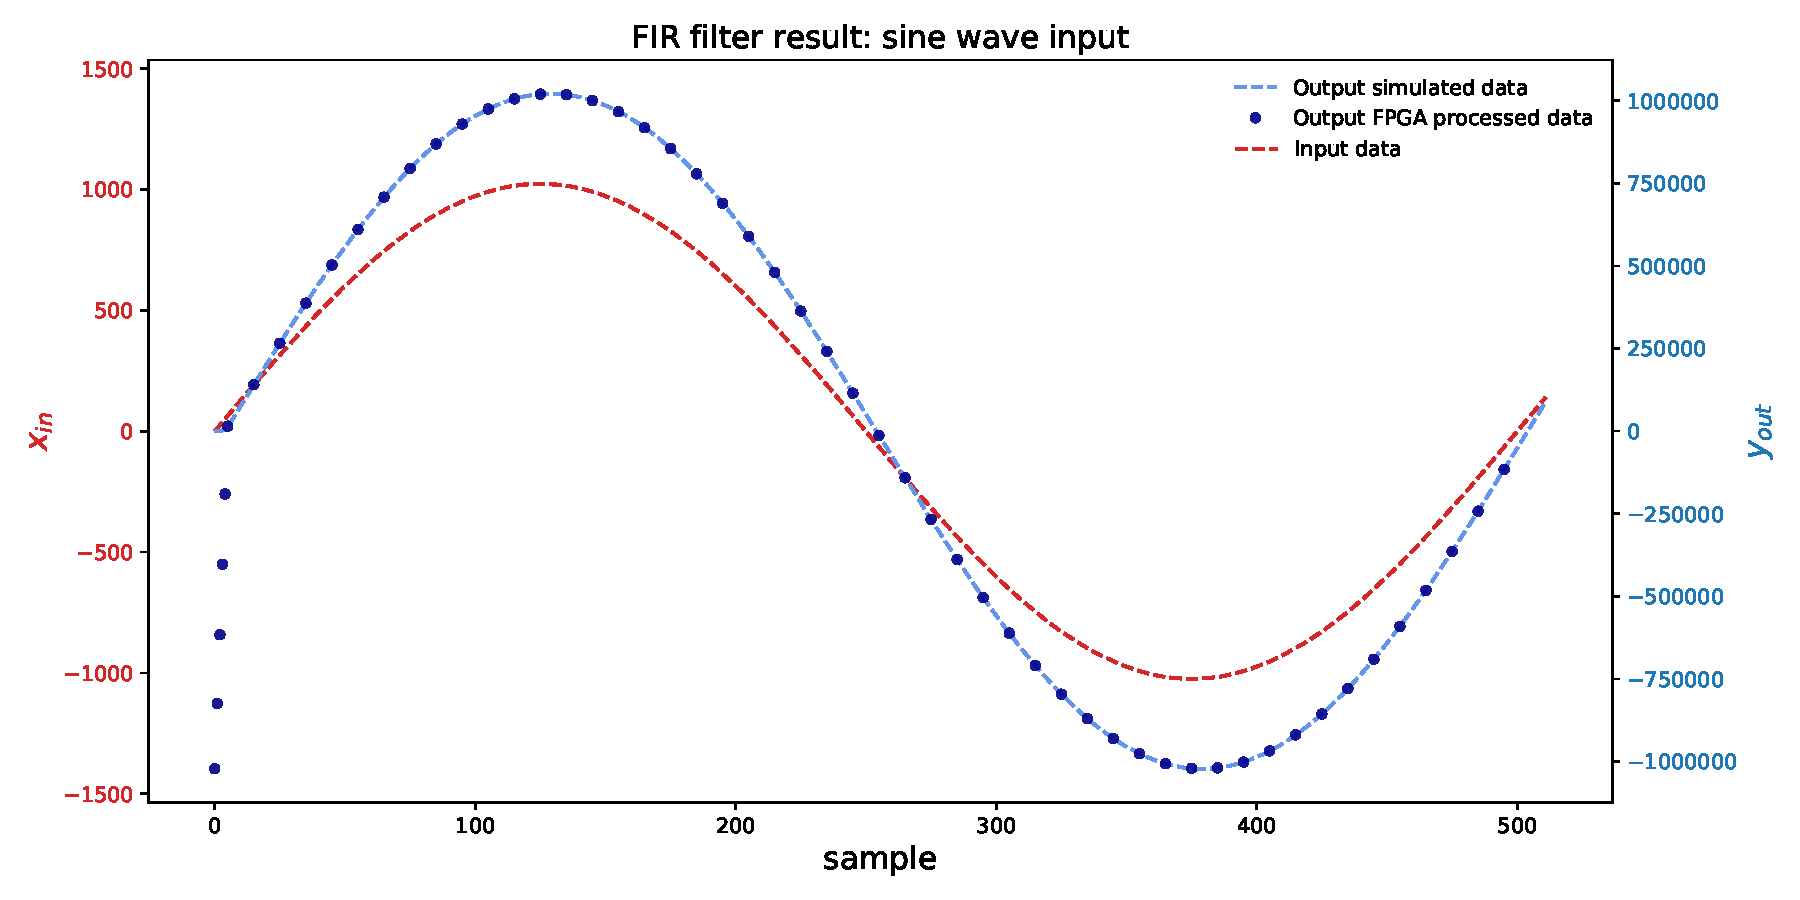
\includegraphics[width=0.65\textwidth]{../images/behavioural/sine.pdf}
    \caption{Results for a sine wave input.}
    \label{fig:sine_wave}
\end{figure}

\subsection{Square wave input}
The second waveform under study is a square wave with the following parameters:
\begin{itemize}
    \item amplitude: $A = 10$;
    \item period: $T = 100 \ \si{samples}$.
\end{itemize}
The results for this waveform are showed in Figure \ref{fig:square_wave}. As before, the plot proves that the filter behaves as expected, except for the initial transient states.

\begin{figure}[h!]
    \centering
    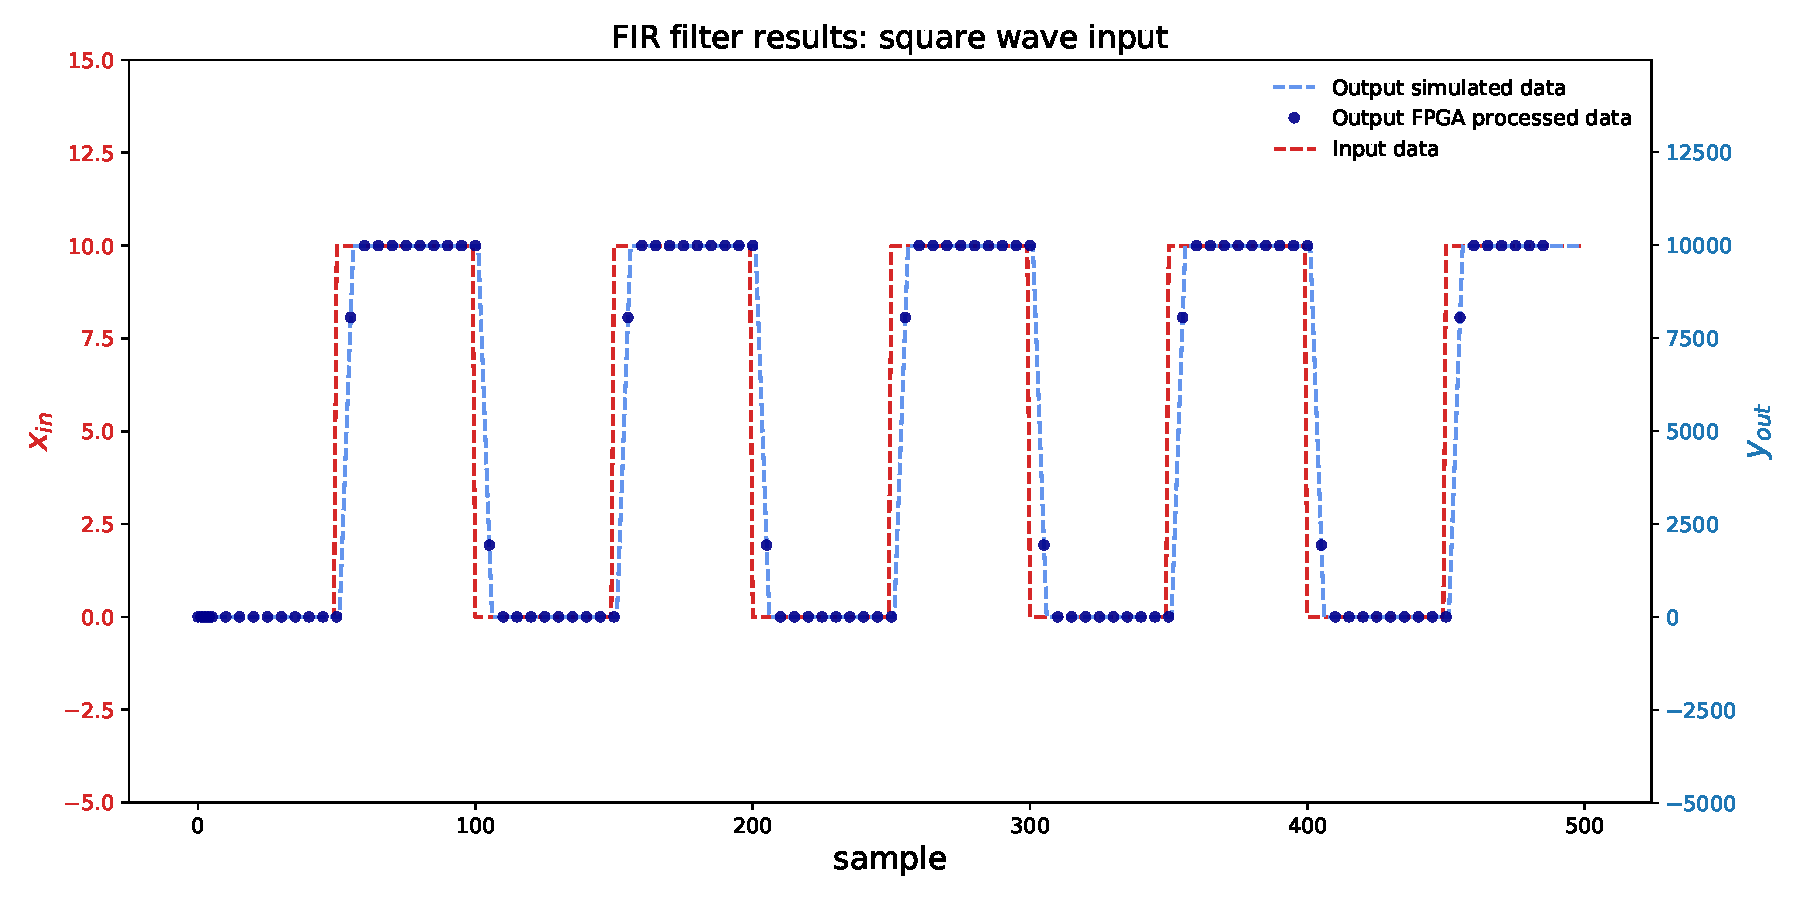
\includegraphics[width=0.65\textwidth]{../images/behavioural/square.pdf}
    \caption{Results for a square wave input.}
    \label{fig:square_wave}
\end{figure}





\section{Conclusion}
In this assignment we present a FIR filter implemented in FPGA hardware. We exploit IPbus protocol and DPRAM for data transferring and storing. 
The system has been experimentally tested on Arty7 board for several input waveforms and results have been compared to the ones obtained from a Python script. In both cases results are coherent, except for the transient states.

\end{document}
